\section{Designing Tests for Creative Writing} \label{sec:approach}
\subsection{Rethinking Torrance Test of Creative Thinking}
Built on J.P. Guilford's work and created by Ellis Paul Torrance, the Torrance Tests of Creative Thinking, a test of creativity, originally involved simple tests of divergent thinking and other problem-solving skills, which were scored on four scales:

\begin{figure*}
\centering
\small
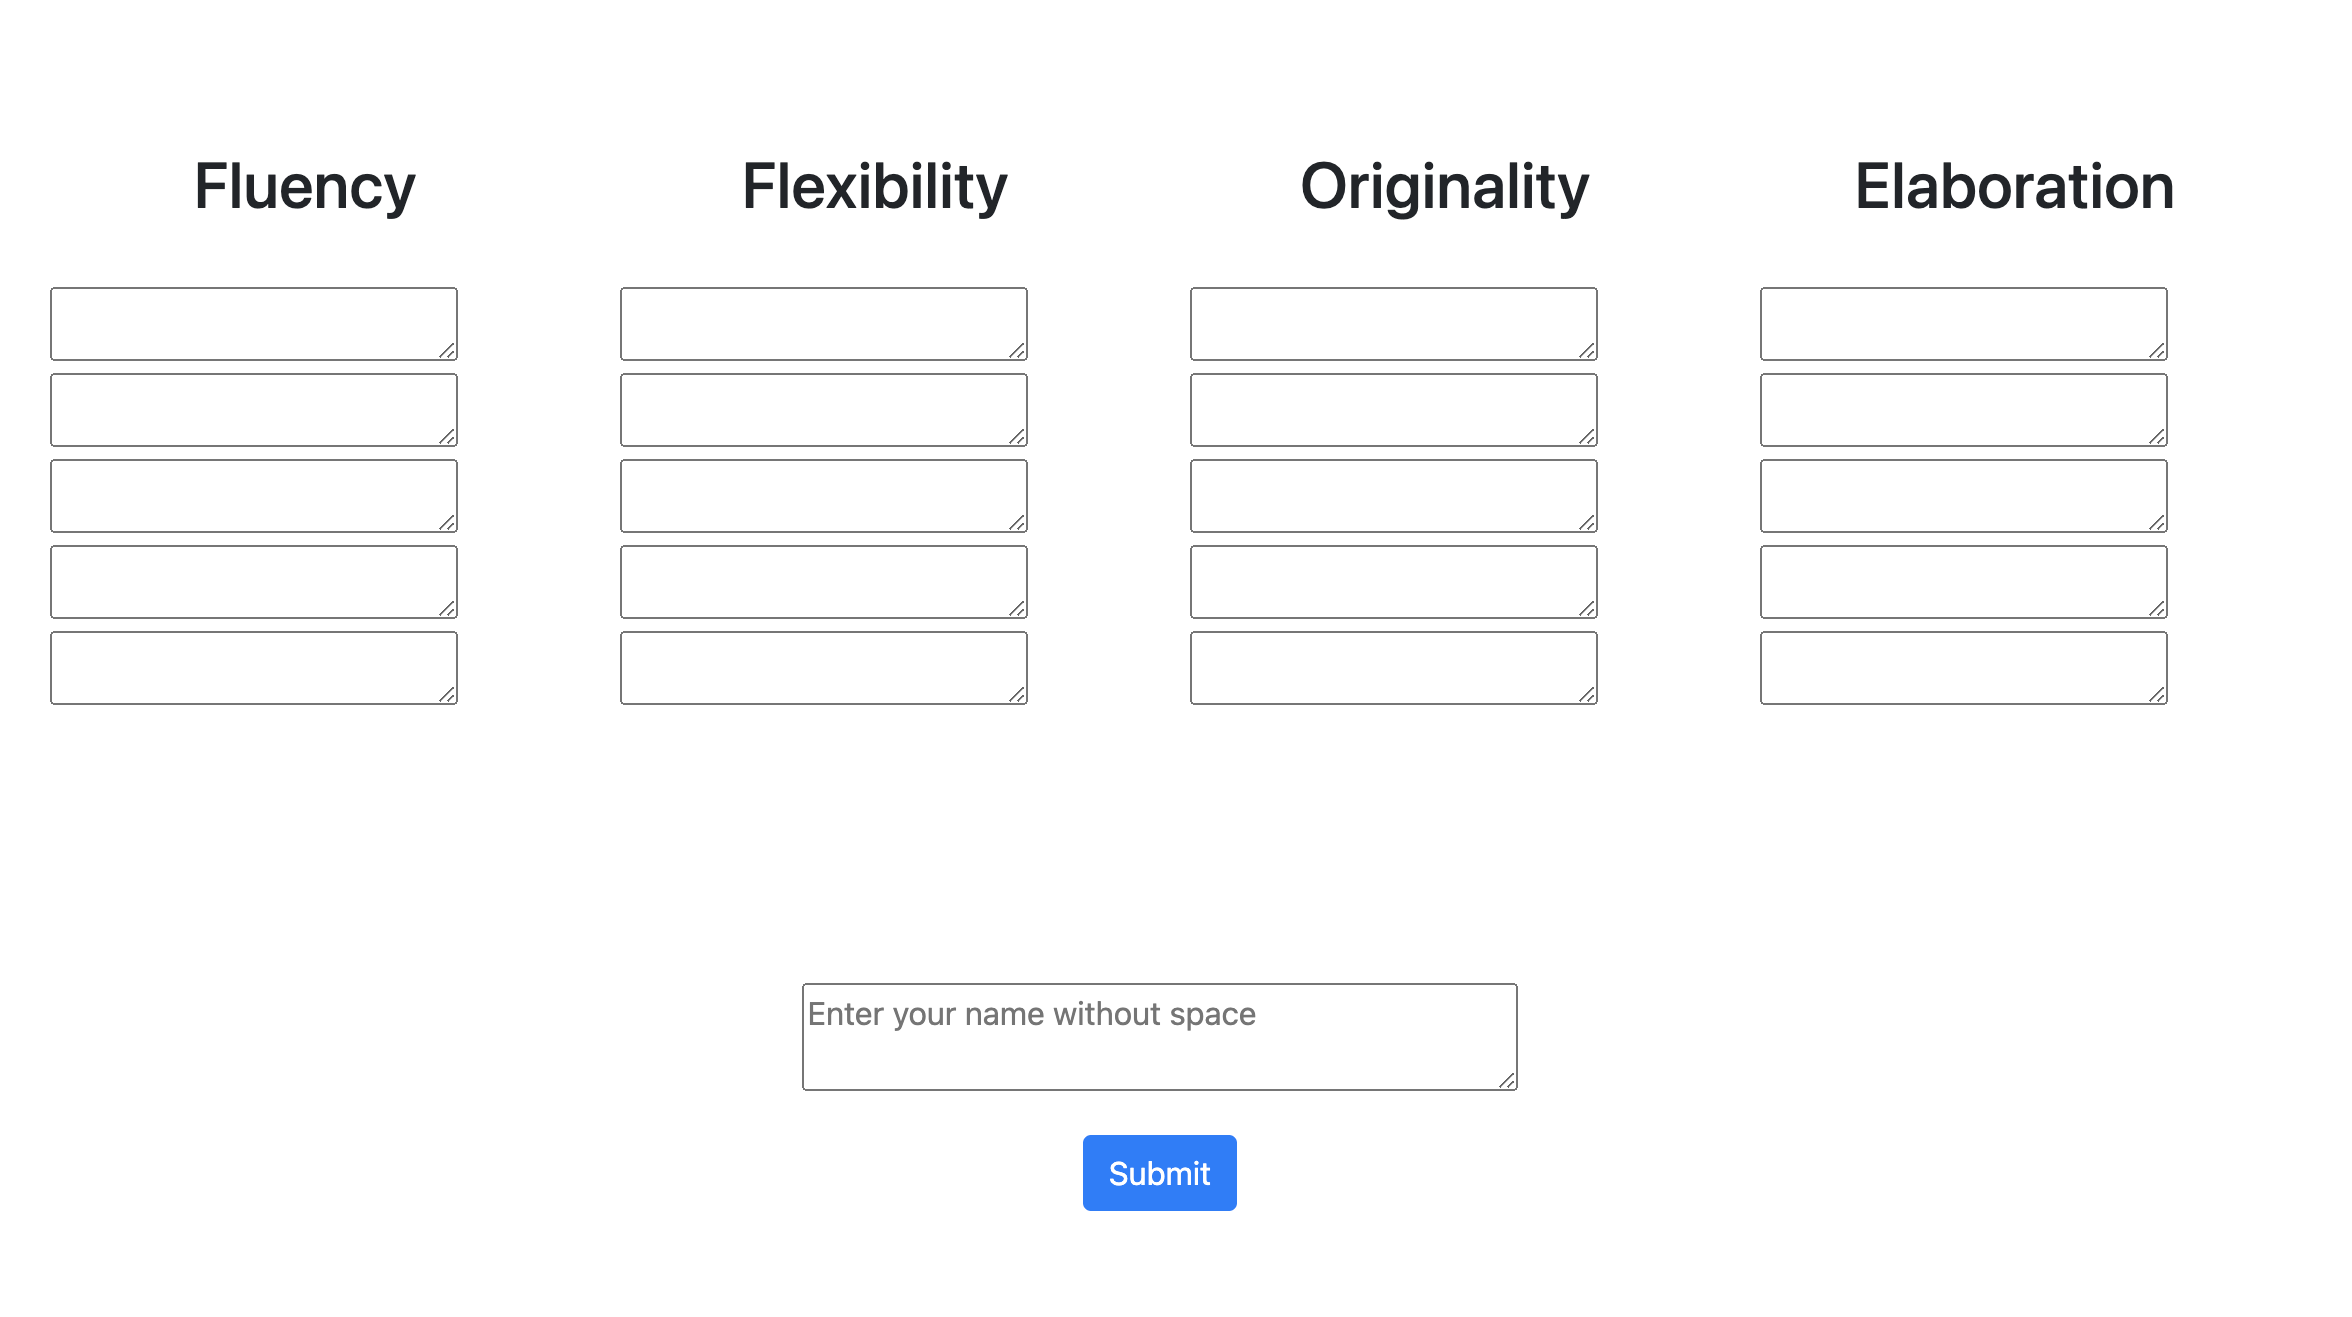
\includegraphics[width=0.8\textwidth]{figures/interface.png}
\caption{\label{fig:interface}Interface to collect Creativity measurements across the four-dimensional analytical framework derived from the Torrance Test of Creative Thinking}
\end{figure*}

\begin{itemize}
    \item Fluency. The total number of interpretable, meaningful, and relevant ideas generated in response to the stimulus.
    \item  Flexibility. The number of different categories of relevant responses.
    \item Originality. The statistical rarity of the responses.
    \item Elaboration. The amount of detail in the responses.
\end{itemize}

While prior work \cite{10.1145/3313831.3376495,10.1145/1978942.1979048,Beketayev2016ScoringDT} has utilized Torrance Test of Creative Thinking in other domains, it hasn't been used to evaluate creative writing. Even though the overall dimensions are generalizable across various forms of art, there are measures specific to creative writing along these dimensions that require the existing definitions to be revised and expanded. For this we recruit experts in creative writing. 

\subsection{Participant Recruitment}
In prior work \cite{gero2023social} has argued that the definition of an ‘expert’ or ‘amateur’ creative writer is difficult in a field that has unclear professional delineations.Though it could be feasible to enlist individuals self-identifying as creative professionals, our requirements necessitated the procurement of participants possessing an intricate and analytical comprehension of the creative writing process. Accordingly, we delimited our participant acquisition to those possessing either a structured educational background in creative writing (for instance, a Master of Fine Arts in Creative Writing), traditionally published authors \footnote{We do not recruit self-published authors}, or lecturers/professors instructing Fiction Writing at the university level.Our recruitment thus resulted in participants who have published novels with leading publishing giants, students enrolled in top MFA programs in the United States, University professors teaching Fiction Writing and screenwriters from prime-time network. Participants were recruited through \textit{User Interviews} (a professional freelancing website) and were paid 70\$ for a taking part in an hour long survey. Table \ref{surveyprof} shows our recruited participants.

\begin{table}[!ht]
\centering
\small
\def\arraystretch{1.35}
\parbox{.45\linewidth}{\begin{tabular}{ll}
\hline
ID & Profession                  \\ \hline
W1 & Professor of Creative Writing \\ \hline
W2 & Professor of Creative Writing \\ \hline
W3 & Lecturer in Creative Writing  \\ \hline
W4 & MFA Fiction Student           \\ \hline
W5 & MFA Fiction Student           \\ \hline
W6 & MFA Fiction Student           \\ \hline
W7 & Author                        \\ \hline
W8 & ScreenWriter                  \\ \hline
\end{tabular}
\vspace{2ex}
\caption{\label{surveyprof}Background of Participants recruited for collecting judgements about Creativity across the dimensions of Torrance Test}
}
\quad\quad\quad\quad
\parbox{.45\linewidth}
{\begin{tabular}{ll}
\hline
Cluster & Participants                  \\ \hline
Narrative Pacing & W4,W6,W7 \\ \hline
\begin{tabular}[c]{@{}l@{}}Understandability\\ \& Coherence\end{tabular}  & W3,W7 \\ \hline
\begin{tabular}[c]{@{}l@{}}Language Proficiency\\ \& Literary Devices\end{tabular}  & W4,W2  \\ \hline
Narrative Ending & W3           \\ \hline
Scene vs Summary & W2,W5,W8          \\ \hline\hline
Structural Flexibility & W3,W7,W8           \\ \hline
Perspective \& Voice Flexibility & W3,W6                        \\ \hline
Emotional Flexibility & W3                  \\ \hline\hline
Originality in Theme/Content & W3                  \\ \hline
Originality in Thought & W1,W2,W3,W5,W7                  \\ \hline
Originality in Form/Structure & W2,W4                  \\ \hline\hline
World Building \& Setting & W2,W6                  \\ \hline
Rhetorical Complexity & W3,W4                  \\ \hline
Character Development & W2,W3,W4,W5,W7,W8                  \\ \hline
\end{tabular}
\vspace{2ex}
\caption{\label{testsource}Background of Participants recruited for collecting judgements about Creativity across the dimensions of Torrance Test}}
\vspace{-5ex}
\end{table}


\subsection{Collecting Creativity Measures}

\begin{table*}[!ht]
\centering
\small
\def\arraystretch{1.5}
\begin{tabular}{|l|l|l|}
\hline
\multirow{5}{*}{Fluency}     & Narrative Pacing                                                                   & \textit{\textbf{\begin{tabular}[c]{@{}l@{}}Does the manipulation of time in terms of compression or stretching\\ feel appropriate and balanced?\end{tabular}}}                                                                                                    \\ \cline{2-3} 
                             & Scene vs Exposition                                                                & \textit{\textbf{\begin{tabular}[c]{@{}l@{}}Does the story display an awareness and insight into the balance \\ between scene and summary/exposition?\end{tabular}}}                                                                                               \\ \cline{2-3} 
                             & \begin{tabular}[c]{@{}l@{}}Language Proficiency \&\\ Literary Devices\end{tabular} & \textit{\textbf{\begin{tabular}[c]{@{}l@{}}Does the story make sophisticated use of idiom or metaphor or\\ literary allusion?\end{tabular}}}                                                                                                                     \\ \cline{2-3} 
                             & Narrative Ending                                                                   & \textit{\textbf{\begin{tabular}[c]{@{}l@{}}Does the end of the story feel natural and earned, as opposed to \\ arbitrary or abrupt?\end{tabular}}}                                                                                                               \\ \cline{2-3} 
                             & \begin{tabular}[c]{@{}l@{}}Understandability \&\\ Coherence\end{tabular}           & \textit{\textbf{\begin{tabular}[c]{@{}l@{}}Do the different elements of the story work together to form a \\ unified, engaging, and satisfying whole?\end{tabular}}}                                                                                              \\ \hline\hline
\multirow{3}{*}{Flexibility} & \begin{tabular}[c]{@{}l@{}}Perspective \& Voice \\ Flexibility\end{tabular}        & \textit{\textbf{\begin{tabular}[c]{@{}l@{}}Does the story provide diverse perspectives, and if there are unlikeable\\ characters, are their perspectives presented convincingly and accurately?\end{tabular}}}                                                    \\ \cline{2-3} 
                             & Emotional Flexibility                                                              & \textit{\textbf{\begin{tabular}[c]{@{}l@{}}Does the story achieve a good balance between interiority and exteriority, \\ in a way that feels emotionally flexible?\end{tabular}}}                                                                                 \\ \cline{2-3} 
                             & Structural Flexibility                                                             & \textit{\textbf{Does the story contain turns that are both surprising and appropriate?}}                                                                                                                                                                          \\ \hline\hline
\multirow{3}{*}{Originality} & Originality in Thought                                 & \textit{\textbf{Is the story an original piece of writing without any cliches?}}                                                                                                                                                                                  \\ \cline{2-3} 
                             & \begin{tabular}[c]{@{}l@{}}Originality in Theme \\ \& Content\end{tabular}                                      & \textit{\textbf{\begin{tabular}[c]{@{}l@{}}Will an average reader of this story obtain a unique and original idea \\ from reading it?\end{tabular}}}                                                                                                              \\ \cline{2-3} 
                             & \begin{tabular}[c]{@{}l@{}}Originality in Form/ \\ Structure\end{tabular}          & \textit{\textbf{Does the story show originality in its form and/or structure?}}                                                                                                                                                                                   \\ \hline\hline
\multirow{3}{*}{Elaboration} & \begin{tabular}[c]{@{}l@{}}World Building \& \\ Setting\end{tabular}               & \textit{\textbf{Does the writer make the fictional world believable at the sensory level?}}                                                                                                                                                                      \\ \cline{2-3} 
                             & Character Development                                                              & \textit{\textbf{\begin{tabular}[c]{@{}l@{}}Does each character in the story feel developed at the appropriate complexity\\ level, ensuring that no character feels like they are present simply to satisfy\\ a plot requirement?\end{tabular}}} \\ \cline{2-3} 
                             & Rhetorical Complexity                                                              & \textit{\textbf{Does the story operate at multiple 'levels' of meaning (surface and subtext)?}}                                                                                                                                                                  \\ \hline
\end{tabular}
\vspace{2ex}
\caption{\label{CreativityTest} Clusters with individual questions to empirically measure creativity across the four dimensions of Torrance Test}
\end{table*}

Following participant enlistment, we explained our objective aimed at assessing creativity in any piece fiction or creative non-fiction, utilizing the four-dimensional analytical framework derived from the Torrance Test of Creative Thinking. Explicit instructions were provided requesting participants to concisely articulate methodologies employed in gauging creativity across these dimensions. In formulating their responses, participants were exhorted to adopt an empirical mindset and eschew abstract or indeterminate terminologies that lack quantifiable attributes. Figure \ref{fig:interface} shows our interface to collect these responses. For each dimension we allowed our participants to state up to 5 measures. We received a total 126 measures from 8 participants across the 4 dimensions. On average each participant provided with 16 measures, 4 for each dimension of creativity.

The measures derived from the involved participants exhibited a considerable degree of semantic congruence. To consolidate these measures from them we prompt GPT-4 \cite{OpenAI2023GPT4TR} to distribute them into individual clusters, each of which encapsulates a generalized representation of a given measure.Each individual cluster was subsequently subjected to a rigorous review by a panel of four domain-specific experts to confirm both the validity of their classification and the comprehensiveness of the represented measures.Measures that could not be quantified empirically at all were discarded.In total we ended up with 14 distinct clusters with 5 representative measures for Fluency and 3 representative measures each for Flexibility, Originality and Elaboration.Some of these measures for creativity came from an individual participant while some measures were uniformly suggested by multiple participants as can be seen in Table \ref{testsource}.

\section{What do these measures tell about Creative Writing?}
Table \ref{CreativityTest} shows the representative measure from each individual cluster across the four dimensions of Creativity.These measures test several aspect of creative writing ranging from originality of thought to well-rounded character development.
\subsection{Fluency}
Compared with both reading and speaking fluency, writing fluency has always been traditionally harder to define \cite{abdel2013we}.Our 5 measures across this dimensions each look at individual aspects of creative writing. 
\subsubsection{Narrative Pacing} 
This measure refers to the manipulation of time in storytelling for dramatic effect. Essentially, it's about controlling the perceived speed and rhythm at which a story unfolds.A skilled writer can manipulate the relationship between these two to affect the pacing of the narrative, either speeding it up (compression) or slowing it down (stretching). This technique plays a crucial role in shaping the reader's experience and engagement with the story. 
\footnote{\url{https://www.writingclasses.com/toolbox/articles/stretching-and-shrinking-time}}
\subsubsection{Scene vs Exposition}
A 'Scene' is a moment in the story that is dramatized in real-time often featuring character interaction, dialogue, and action while 'Exposition', on the other hand, involves summarizing events or providing information like character history, setting details, or prior events. The right balance between scene and summary/exposition can vary depending on the story, but in general, it's essential for maintaining a good pace, keeping the reader engaged, and delivering necessary information \cite{burroway2019writing}. 
\footnote{\url{https://creativenonfiction.org/syllabus/scene-summary/}}
\subsubsection{Language Proficiency \& Literary Devices} 
Eminent novelist Milan Kundera said ``\textit{Metaphors are not to be trifled with. A single metaphor can give birth to love.}". Sophisticated use of literary allusion or figurative language such as metaphor/idioms often add depth, interest, and nuanced meaning to any creative writing. It allows for a richer reading experience, where the literal events are imbued with deeper symbolic or thematic significance. 
\subsubsection{Narrative Ending}
In her New Yorker essay ``On Bad Endings" \cite{BadEndings} Joan Accocela writes 
            \begin{quote}
                \centering
                ``Another possibility is that the author just gets tired. I review a lot of books, many of them non-fiction. Again and again, the last chapters are hasty and dull. `I’ve worked hard enough,' the author seems to be saying. `My advance wasn’t much. I already have the idea for my next book. Get me out of here.'"
            \end{quote}
If the writer ends the piece simply because they are ``tired of writing", the conclusion might feel abrupt, disjointed, or unfulfilling to the reader. This is one of the important factors of creative writing fluency.A strong ending offers a sense of closure, ties up the central conflicts or questions of the story, and generally leaves the reader feeling that the narrative journey was worthwhile and complete.
\subsubsection{Understandability \& Coherence}
Narrative coherence is the degree to which a story makes sense  \footnote{https://en.wikipedia.org/wiki/Narrative\_paradigm}.A well-crafted story usually follows a logical path, where the events in the beginning set up the middle, which then logically leads to the end. Every scene, character action, and piece of dialogue should serve the story and propel it forward. Well-written stories have an underlying unity that binds the elements together. The themes, plotlines, character arcs, and other elements of the story interweave to create a harmonious whole. A story with `disorder' might feel disjointed, with characters, scenes, etc that don't connect or contribute to the overall narrative.

\subsection{Flexibility}
Flexibility is often referred to as the ability to look at something from a different angle or point of view. In the context of creative writing our participants agreed on 3 distinct measures of Flexibility
\subsubsection{Perspective \& Voice Flexibility}
An \textit{omniscient} narrator is the all-knowing voice in a story that can convincingly and accurately depict a wide range of character viewpoints, including those of characters who may be morally ambiguous, difficult, or otherwise unappealing. This can also potentially involve diving into the mindset of characters who may act or think in ways that the reader, or even the writer, finds objectionable or repugnant.As stated in \cite{friedman1955point} an omniscient narrator enhances a sense of reliability or truth within literary works since readers are given deeper insights into many characters. The multiple viewpoints feel more objective because readers have access to multiple interpretations of events and can thus decide how they feel about each character’s perspective.
\subsubsection{Emotional Flexibility}
Emotional flexibility is asking whether the piece of writing effectively balances action and introspection, and if it portrays a broad and realistic spectrum of emotions. \textit{Exteriority} refers to the observable actions, behaviors, or dialogue of a character, and the physical or visible aspects of the setting, plot, and conflicts.\textit{Interiority}, on the other hand, pertains to the inner life of a character — their thoughts, feelings, memories, and subjective experiences. A balance between these two aspects is crucial in creating well-rounded characters and compelling narratives. As stated in \cite{campe2014rethinking} if a story is too heavy on exteriority, it may feel shallow or lack emotional depth. If it leans too much on interiority, it could become overly introspective and potentially lose the momentum of the plot.
\subsubsection{Structural Flexibility}
A good piece of creative writing often has plot twists, character developments, or thematic revelations that surprise the reader, subverting their expectations in a thrilling way. It's about keeping readers engaged and curious, never fully knowing what's going to happen next. However despite the surprises and twists, the turns in the story must also make sense within the established context of the story's universe, its characters, and its themes. This means that even though an event might be surprising, it should feel appropriate or fitting in hindsight. It shouldn't feel like the writer has broken the rules they've set up, or made a character behave inconsistently without reason, simply for the sake of shock value.
\subsection{Originality}
Creative writing requires originality, or the ability to generate unique ideas \cite{ward1999creative}. Originality can conveyed in several ways. Our participants suggested three unique ways in which they look for originality in creative writing.
\subsubsection{Originality in Theme and Content}
In his book ``Literature and the Brain" well-known literary critic and scholar Norman Holland discusses how stories stimulate the mind and impact readers \cite{holland2009literature}. A good story that offers a deeper understanding of human nature, cultural insights,unique viewpoints, or even the exploration of new ideas and themes has a lasting impact on its reader and society .It is meant to entertain, inform, provoke thought, challenge beliefs, provide comfort, or raise awareness on specific issues.In ``Poetic Justice", prominent philosophers Martha Nussbaum explores how the literary imagination is an essential ingredient of public discourse and a democratic society \cite{nussbaum1997poetic}.As such originality in theme and content is an important measure of creative writing.
\subsubsection{Originality in Thought}
A cliche is an idea, expression, character, or plot that has been overused to the point of losing its original meaning or impact \cite{fountain2012cliches}. They often become predictable and uninteresting for the reader.In his book \cite{clark2008writing} eminent American writer, editor, and a writing coach: Roy Peter Clark advised writers to strictly avoid cliches because they often indicate a lack of original thought or laziness in language use.Originality suggests that the piece isn't cliche.
\subsubsection{Originality in Form/Structure}
In his book \cite{boardman1992narrative} Michael M. Boardman discusses how innovation in narrative structure can serve ideological purposes and challenge conventional narrative forms. Frederic Jameson  highlighted the complexities of postmodern literature, where the blurring of genres and innovation in form and structure was a key characteristic\cite{jameson1991postmodernism}. Originality in form/structure has also been accomplished by unconventional use of format, genre or plot structure.For instance, the Pulitzer winning book \textit{The Color Purple} from Alice Walker is told through a series of letters written by the protagonist. Neil Gaiman's \textit{American Gods} on the other hand combines elements of fantasy, mystery, and mythic fiction in unexpected ways. \textit{The Sound and the Fury} by William Faulkner deviates from the traditional plot structure by presenting a narrative that unfolds through the stream of consciousness of different characters. The goal of originality in form or structure is often to provide a fresh reader experience, challenge conventional reading expectations, or to create a deeper or more complex exploration of the story's themes.
\subsection{Elaboration}
\subsubsection{World Building and Setting}
American poet and memoirist Mark Doty discusses the importance of create a vivid, immersive reality at the sensory level through the use of detailed, evocative description \cite{doty2014art84794531}.An effective writer often uses sensory details to paint a detailed picture of the story's environment, making it feel tangible and real to the reader.For example, describing the specific colors and shapes in a scene, the sounds that fill a space, the textures and temperatures that a character comes into contact with, the flavors of the food they eat, or the scents that fill the air, can all contribute to creating a sensory-rich and believable world.By stimulating the reader's senses, the writer can make the reader feel as though they're experiencing the events of the story firsthand. This level of detail contributes to the believability of the world, even if it's a completely fictional or fantastical setting. It helps the reader to suspend disbelief and become more deeply invested in the narrative.
\subsubsection{Character Development}
A 'flat character' is typically a minor character who is not thoroughly developed or who does not undergo significant change or growth throughout the story. They often embody or represent a single trait or idea, and they're only used to advance the plot or highlight certain qualities in other characters. A 'complex character' on the other hand also known as a round character, has depth in feelings and passions, has a variety of traits of a real human being, and evolves over time. They have their strengths, weaknesses, and they learn from their experiences. \cite{forster1927aspects,fishelov1990types,currie1990nature} highlights that any creative piece of fiction or non-fiction tend to be more engaging to the reader when authors can take a character who initially appears to be one-dimensional or stereotypical (flat) and add depth to them, as it mirror the complexity of real people.
\subsubsection{Rhetorical Complexity}
In Ernest Hemingway's short story "Hills Like White Elephants," the couple's conversation about seemingly unrelated topics implies a much deeper and more serious discussion about an abortion. Their actual dialogue never directly addresses this issue, but it's heavily suggested through what's left unsaid — the subtext. Effective writing often operates on both surface and subtext levels. The surface text keeps the reader engaged with the plot and characters, while the subtext provides depth, complexity, and additional layers of interpretation, contributing to a richer and more rewarding reading experience \cite{kochis2007baxter,phelan1996narrative}.

